\documentclass{beamer}
\usepackage[utf8]{inputenc}
\usepackage[T1]{fontenc}
\usepackage{lmodern}
\usepackage{ngerman}
\usepackage{bibgerm}
\usepackage{color}
\usepackage{graphicx}
\usepackage{pstricks}

\mode<presentation>  {
  \usetheme{Warsaw}
  \useoutertheme{miniframes}
  \setbeamertemplate{navigation symbols}{}
}

\newcommand{\defaultscale}{0.5}
\newcommand{\pfeil}{\item[$\Rightarrow$]}

\title[MagicL]{MagicL: Ein S-Expression-basiertes Framework für
  Compiler-Konstruktion nach dem Baukastenprinzip}
\subtitle{Diplomarbeit}
\author{Benjamin Teuber}
\date{\today}
\institute{Universität Hamburg\\ 
  Fakultät für Mathematik, Informatik und Naturwissenschaften\\
  Department Informatik\\
  AOSE'08}

\begin{document}
\maketitle

\section{Einführung}
\subsection{}

\begin{frame}{Themengebiet}
  \begin{itemize}
  \item Buzzwords:
    \begin{itemize}
    \item Model-driven architecture
    \item Domain-specific languages
    \item Metaprogramming
    \end{itemize}
  \item Problem: Compiler bauen ist aufwändig
    \begin{itemize}
    \item Parser für Quellsprache
    \item Compiler in normalaler Programmiersprache
    \item Templates für Zielsprache
    \end{itemize}
  \item Wie können wir das vereinfachen?
  \pfeil Lightweight-Compiler
  \end{itemize}
\end{frame}

\section{Lisp}
\subsection{}

\begin{frame}{Exkursion: Lisp}
  \begin{itemize}
  \item Eine der ältesten Programmiersprachfamilien (LISP: 1958)
  \item Minimale, uniforme Syntax (S-Expressions $\simeq$ XML-Subset)
  \item Sprache selbst kann durch Makros erweitert werden (``The
    programmable programming language'')
  \end{itemize}

  \begin{block}{}
    ``Any sufficiently complicated C or Fortran program contains an ad hoc
    informally-specified bug-ridden slow implementation of half of
    Common Lisp.''

    - Philip Greenspun
  \end{block}
\end{frame}

\begin{frame}[fragile]{S-Expressions}
  \begin{itemize}
  \item Ein S-Expression ist entweder:
    \begin{itemize}
    \item Ein Atom, z.B. eine Zahl, ein String, eine Variable
    \item Eine Liste von S-Expressions in Notation \\ \texttt{($sexp_1$ $sexp_2$ .. $sexp_n$)}
    \end{itemize}
  \item S-Expressions werden nach dem Parsen \textit{strukturell} gespeichert.
  \item Beipiel: Funktionsdefinition in Common Lisp
  \end{itemize}
\begin{verbatim}
(defun my-add (a b)
  (+ a b))
\end{verbatim}
\end{frame}

\begin{frame}{Lisp-Makros}
  \begin{itemize}
  \item Makros sind Funktionen von Code nach Code
  \item werden bereits beim Compilieren ausgewertet
  \item Ermöglichen inkrementelle Erweiterung des Lisp-Compilers
  \item Vergleich: Präprozessor in C
    \begin{itemize}
    \item Arbeiten auf S-Expressions einfacher \& mächtiger
    \item Volle Lisp-Funktionalität steht zur Verfügung
    \pfeil Probleme wie Namenskonflikte können elegant gelöst werden
    \end{itemize}
  \end{itemize}
\end{frame}

\begin{frame}[t, fragile]{Lisp-Makros (2)}
  \begin{itemize}
  \item Beispiel: Eigenes \texttt{switch} durch \texttt{if} ausdrücken
  \end{itemize}
  \begin{block}{Macro-Eingabe}
\begin{verbatim}
(switch input
  ("Hallo"      (print "Hallo auch"))
  ("Tschüss"    (print "Bye Bye"))
  ("Wie gehts?" (print "Gut soweit")))
\end{verbatim}
  \end{block}
  \begin{block}{Erzeugter Code}
\begin{verbatim}
(if (== input "Hallo")
  (print "Hallo auch")
 elseif (== input ""Tschüss") 
  (print "Bye Bye")
 elseif (== input "Wie gehts?")
  (print "Gut soweit"))
\end{verbatim}
  \end{block}
\end{frame}

\begin{frame}{Warum Makros toll sind}
  \begin{itemize}
  \item Compiler nicht als monolithischer Block
  \item Statt dessen Bauskastenprinzip
  \item Interface für nachträgliche Erweiterungen durch den User
  \item ``Embedded DSLs'' - in die ursprüngliche Sprache integriert
  \item Alles S-Exp-basiert: Parser \& Generator fallen weg
  \item Lisp bietet praktische DSL für Makro-Definitionen 
  \end{itemize}
\end{frame}

\section{Diplomarbeit}
\subsection{Diplomarbeit}

\begin{frame}{Motivation der Diplomarbeit}
  \begin{itemize}
  \item Idee: Übernehmen des Lisp-Ansatzes für beliebige Computersprachen, z.B.
    \begin{itemize}
    \item Java
    \item VHDL
    \item HTML
    \item Latex
    \item POV-Ray
    \end{itemize}
  \pfeil Einheitliche Syntax, einheitliche IDE, einheitliche Erweiterungsmöglichkeiten
\end{itemize}
\end{frame}

\begin{frame}{Ziel der Diplomarbeit}
  \begin{itemize}
  \item Entwurf eines S-Expression-basierten Compilerbau-Frameworks
  \item Integrierte DSLs für:
    \begin{itemize}
    \item Generatoren: Compilieren S-Exp-Sprachen in Quellcode einer Backend-Sprache
    \item Compiler: Übersetzen eine S-Exp-Sprache in eine andere
    \item Parser: Lesen externen Quelltext ein und erzeugen S-Expressions
    \end{itemize}
  \item Default-Parser für S-Expressions
  \end{itemize}
\end{frame}

\begin{frame}{Erster Prototyp}
  \begin{itemize}
  \item Ca. ein Jahr alt - proof of concept
  \item Nachbildung des Lisp-Makroprozessors
  \item In Ruby geschrieben
  \item Zwei Sexp-Sprachen:
    \begin{itemize}
    \item Ruby - kompiliert nach Ruby-Quellcode
    \item Compiler - DSL für Sprachdefinitionen, kompiliert nach Ruby-Sexp
    \end{itemize}
  \item Seit dem erfolfreichen \textit{bootstrapping} nur noch
    generierter Ruby-Code
  \end{itemize}
\end{frame}

\begin{frame}{Neue Version}
  \begin{itemize}
  \item Derzeit im entstehen
  \item In (generiertem) Haskell programmiert - der Sprache für ``theorienahe Anwendungen''
  \item Eigener Ansatz zum Compilerbau statt Makro-Nachbau
    \begin{itemize}
    \item Mathematisch fundiert: Kategorientheorie
    \item Operatoren wie in EBNF möglich
    \end{itemize}  
  \end{itemize}
\end{frame}

\section{Kategorientheorie}
\subsection{Kategorientheorie}

\begin{frame}{Kategorientheorie}
  \begin{itemize}
  \item Kategorientheorie
    \begin{itemize}
    \item Sehr abstrakter Bereich der Mathematik
    \item Praktisch alle mathematischen Strukturen sind Kategorien
    \end{itemize}
  \item Grundidee
    \begin{itemize}
    \item Abstraktion von Funktionstypen
    \item Komposition von Funktionen
    \end{itemize}
  \end{itemize}
  \begin{figure}
    \centering
    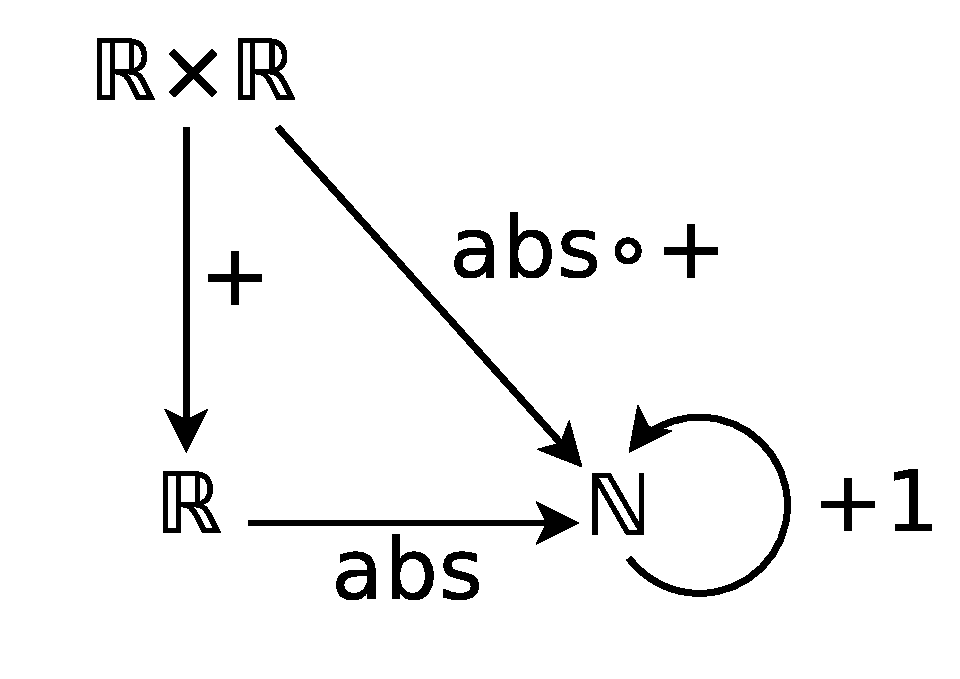
\includegraphics[scale=0.3]{images/cat_funs}
    \caption{Ein simples Funktionensystem}
  \end{figure}
\end{frame}

\begin{frame}{Nun formal}
  \begin{itemize}
  \item Eine Kategorie $C = (Ob, Mor, \circ, id)$ besteht aus  
    \begin{itemize}
    \item einer Klasse $Ob$ von Objekten
    \item einer Menge Morphismen $Mor_{A,B}$ zu je zwei Objekten $A, B$
      ($A$ wird Quelle genannt, $B$ Ziel)
    \item einem Kompositionsoperator $\circ_{A,B,C}$ zu je drei Objekten
      $A, B, C$ mit 
      $\circ_{A,B,C} : Mor_{B,C} \times Mor_{A,B} \rightarrow Mor_{A,C}$
    \item einer Identität $id_A \in Mor_{A,A}$ für jedes Objekt $A$ mit
    \end{itemize}
  \item Axiome:
    \begin{itemize}
    \item Assoziativität von $\circ$:
      $f \circ (g \circ h) = (f \circ g) \circ h$
    \item Verträglichkeit mit Identität:
      $f \circ id_A = id_B \circ f = f$ für $f \in Mor_{A,B}$
    \end{itemize}
  \end{itemize}
\end{frame}

\begin{frame}{Eine einfache Kategorie}
  \begin{figure}
    \centering
    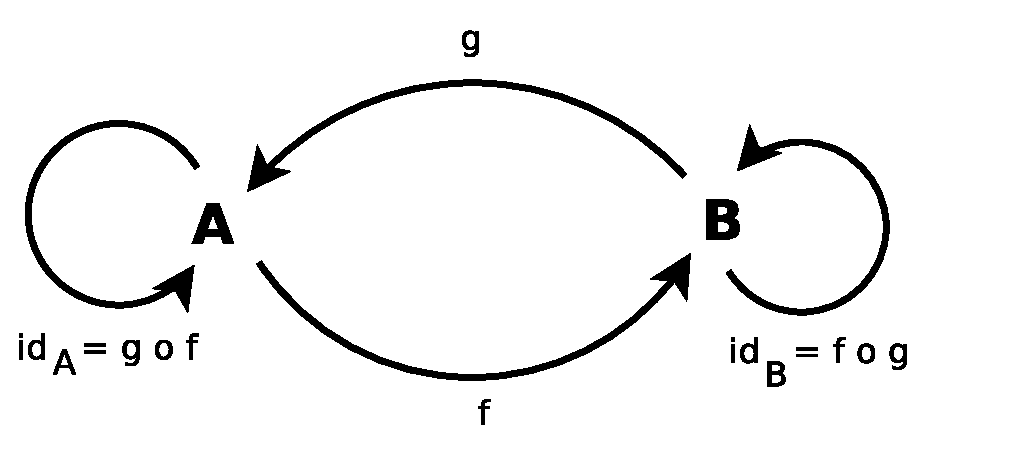
\includegraphics[scale=0.4]{images/cat_simple}
    \caption{Eine einfache Kategorie}
  \end{figure}
  \begin{itemize}
  \item Diese simple Kategorie besteht aus
    \begin{itemize}
    \item zwei Objekten $A, B$
    \item vier Morphismen $f, g, id_A, id_B$
    \end{itemize}
  \item Alle Kompositionen ergeben wieder einen der vier Morphismen
  \end{itemize}
\end{frame}

\begin{frame}{Abbildungen zwischen Kategorien: Funktoren}
  \begin{itemize}
  \item Ein Funktor $F$ von Kategorie $C$ nach Kategorie $D$
    \begin{itemize}
    \item bildet Objekte auf Objekte ab
    \item bildet Morphismen aus $Mor_{A,B}$ auf Morphismen aus
      $Mor_{F(A),F(B)}$ ab 
    \end{itemize}   
  \item Muss mit Komposition und Identität verträglich sein:
    \begin{itemize}
    \item $F(f \circ g) = F(f) \circ F(g)$
    \item $F(id_A) = id_{F(A)}$
    \end{itemize}
  \end{itemize}   
\end{frame}

\begin{frame}{Produkte}
  \begin{itemize}
  \item Entspricht kartesischen Produkt
  \item Benötigt keine Mengen zur Definition!
  \item Idee: Projektionen und sog. "`Mittler-Morphismus"'
  \end{itemize}
  \begin{figure}
    \centering
    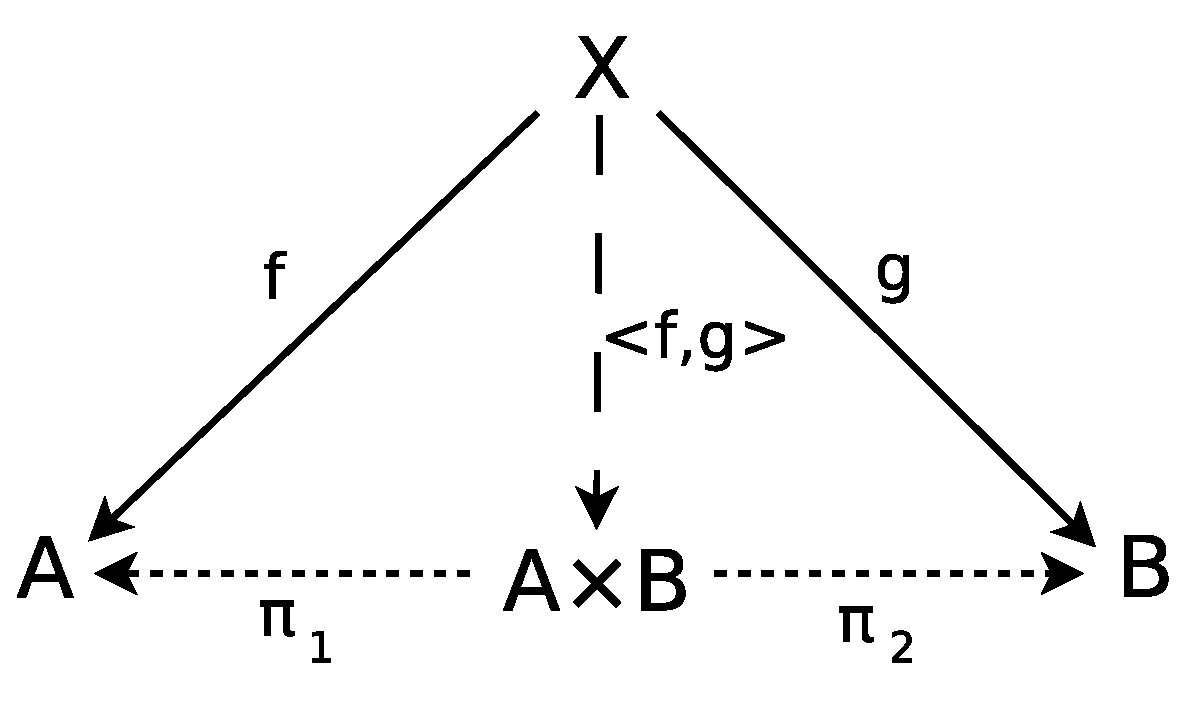
\includegraphics[scale=0.3]{images/cat_product}
    \caption{Produkt-Diagramm}
  \end{figure}
\end{frame}

\begin{frame}{Coprodukte / disjunkte Summen}
  \begin{itemize}
  \item "`Umkehrung"' vom Produkt
  \item $A + B$ entspricht einer disjunkten Summe von $A$ und $B$
  \end{itemize}
  \begin{figure}
    \centering
    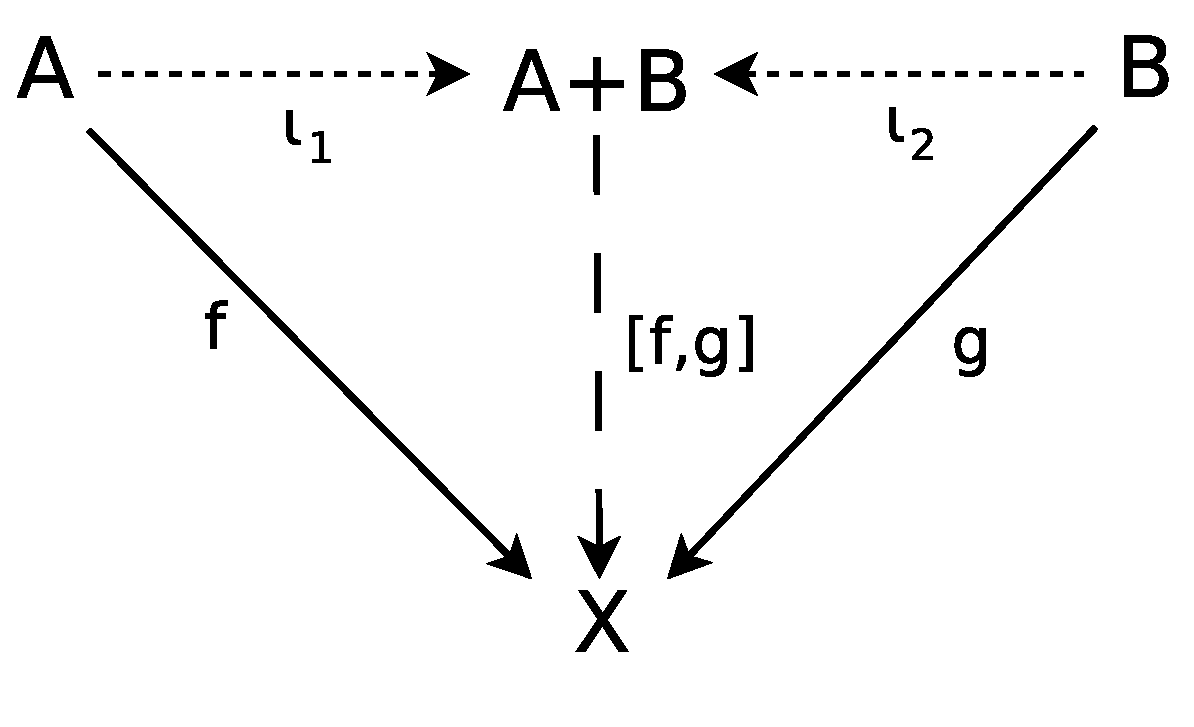
\includegraphics[scale=0.3]{images/cat_coproduct}
    \caption{Coprodukt-Diagramm}
  \end{figure}
\end{frame}

\begin{frame}{Kategorien in dieser Arbeit}
  \begin{itemize}
  \item Hier immer: Haskell-Datentypen als Objekte
  \item Arrows variieren:
    \begin{itemize}
    \item pure Funktionen (Kategorie $Hask$)
    \item Funktionen mit Side-Effects
    \item Bestehende Arrows mit versteckten Ein- und Ausgaben
    \end{itemize}
  \end{itemize}
\end{frame}

\begin{frame}{Ziel: Eine Parser-Kategorie}
  \begin{itemize}
  \item Eigenschaften von Parsern:
    \begin{itemize}
    \item Können fehlschlagen und Alternativen ausdrücken
    \item Besitzen einen Zustand (Position im Eingabestream)
    \end{itemize}
  \item Plan: Bestehende Kategorien um Fehlschlagen / Zustände erweitern \\
  $\Rightarrow$ Funktoren
  \end{itemize}
\end{frame}

\begin{frame}{Der Funktor Fail}
  \begin{itemize}
  \item Nun zwei Möglichkeiten für Rückgabe:
    \begin{itemize}
    \item Scheitern (Rückgabe einer Fehler-Nachricht)
    \item Erfolg (normaler Rückgabewert)
    \end{itemize}
  \item Verstecken der Veränderung: Neue Kategorie $C_{f}$
  \item $f_{f} : A \rightarrow B$ wird abgebildet auf
    $f : A \rightarrow String + B$
  \item Der Arrow $fail_{f} : String \rightarrow a$ in $C_{f}$ schlägt immer
    fehl und entspricht $fail : String \rightarrow String + a$ in $C$
  \item Der Operator $\bigvee : Mor_{A,B} \times Mor_{A,B} \rightarrow
    Mor_{A,B} $ bietet Alternativen
  \end{itemize}
\end{frame}

\begin{frame}{Der Funktor Fail (2)}
  \begin{itemize}
  \item Komposition in $C_{f}$:  $g_{f} \circ f_{f} = ([fail,g] \circ f)_{f}$ 
  \end{itemize}
  \begin{figure}
    \centering
    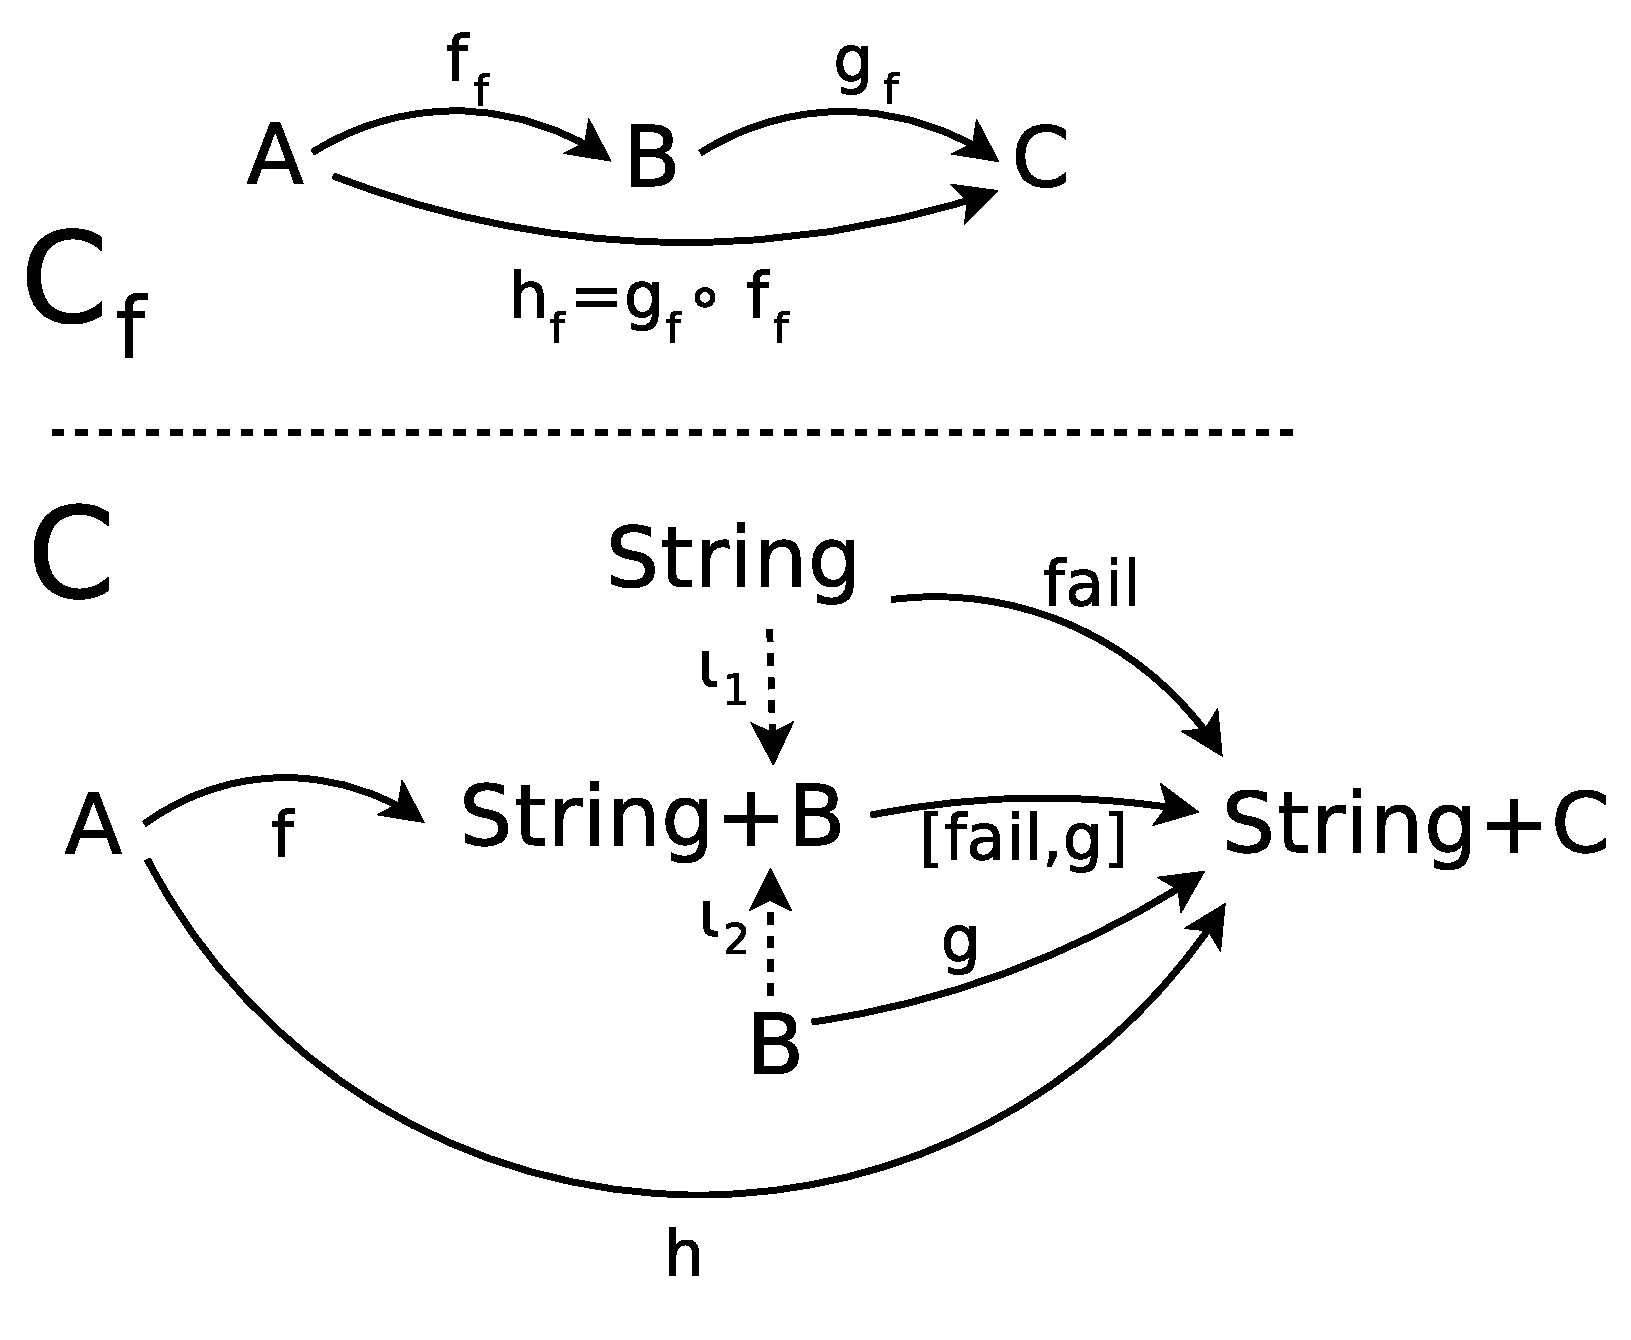
\includegraphics[scale=0.3]{images/cat_fail}
    \caption{Komposition beim Fail-Funktor}
  \end{figure}
\end{frame}

\begin{frame}{Der Funktor State}
  \begin{itemize}
  \item Nun sollen Zustände vom Typ S weitergereicht werden
  \item Wieder verstecken, neue Kategorie $C_{s}$ mit Funktor
    $State : C_{s} \rightarrow C$
  \item $f_{s} : A \rightarrow B$ wird abgebildet auf
    $f = A \times S \rightarrow B \times S$
  \item Komposition in $C_{s}$ einfach
    \begin{figure}
      \centering
      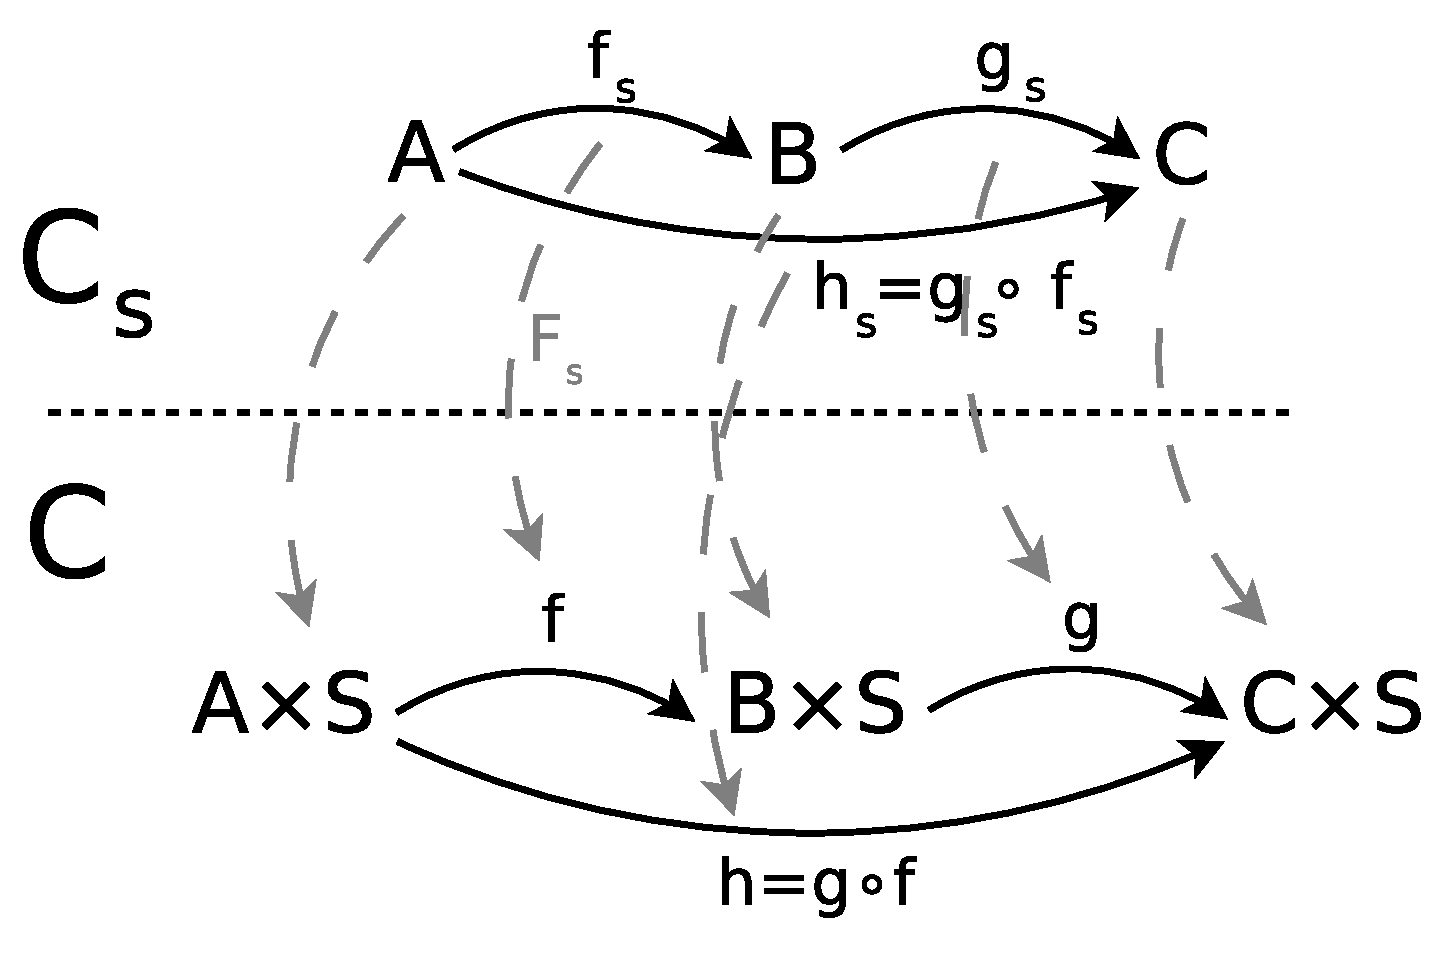
\includegraphics[scale=0.2]{images/cat_state}
      \caption{Komposition beim State-Funktor}
    \end{figure}
  \end{itemize}
\end{frame}

\begin{frame}{Der Funktor State (2)}
  \begin{itemize}
  \item Etwas Tricky: Produkte in $C_{s}$
  \item Arbeiten mit Zuständen: Lesen \& Schreiben:
  \item Lesen: $get_s : \forall a : a \rightarrow S$
  \item Schreiben: $put_s : S \rightarrow *$
  \item Zum Parsen: $S = List$ $of$ $T$ mit Token-Typ $T$
  \end{itemize}
\end{frame}

\begin{frame}{Der Parse-Funktor}
  \begin{itemize}
  \item Kombination von Fail und State zu einem Funktor Parse
  \item $C_p = C_{ffs}$
  \item Zwei Fail-Funktoren für bessere Fehlermeldungen
  \item Beispiel:
    \begin{itemize}
    \item Grammatik: \texttt{\{.*\} $\bigvee$ [.*]}
    \item Eingabewort: \texttt{\{ABC}
    \item Schlecht: \texttt{"'Expected [, got \{"'}
    \item Gut: \texttt{"'Expected \}, got end of stream"'}
    \item Scheitern nach \texttt{\{} soll Backtracking aushebeln \\
      $\Rightarrow$ \textit{innerer Fail}
    \end{itemize}
  \end{itemize}
\end{frame}

\begin{frame}{Der Parse-Funktor (2)}
  \begin{itemize}
  \item Flexible Parser-Anwendungen dank Funktor
    \begin{itemize}
    \item Funktionale Parser: $Hask_p$
    \item Parser mit Side-Effects: $IO_p$
    \item Parser mit anderen Extras: Weitere Funktoren möglich
    \end{itemize}
  \item Token-Typ Variabel:
    \begin{itemize}
    \item \texttt{Char} für Textdateien
    \item \texttt{Bool} für Bytestreams
    \item \texttt{Sexp} für S-Expressions
    \end{itemize}
  \item Parser-Bibliothek enthält dazu:
    \begin{itemize}
    \item Praktische Funktionen zum Parser-Erzeugen (Blick in \texttt{Parser.hs})
    \item Möglichkeiten zum Aufruf von inneren Parsern
    \item Konzepte zum Verschalten von Parsern und Compilern
    \end{itemize}
  \end{itemize}
\end{frame}

\begin{frame}{Parsen von S-Expressions}
  \begin{itemize}
  \item Besonderheit: Token können selbst Listen sein
  \item Lösung: Als Stream behandeln, \texttt{compNode} wendet Parser
    auf inneren Stream an
    \begin{itemize}
    \item Beispiel: Lesen von \texttt{(hallo welt)}
    \item \texttt{compNode (symeq "'hallo"' >>> symeq "'welt"') } % <<
    \end{itemize}
  \item Makros: \texttt{compNode mit Prüfung des ersten Symbols}
    \begin{itemize}
    \item obiges Beispiel: \texttt{macro "'hallo"' (symeq "'welt"')}
    \item Stimmt das erste Symbol überein, wird das Backtracking aufgehoben
    \end{itemize}
  \end{itemize}
\end{frame}

\section{Schluss}
\subsection{Schluss}

\begin{frame}{Beispiel-Code}
  \begin{itemize}
  \item Sexp-Parser (liest Text)
  \item Haskell-Parser (liest Sexp)
  \item Arrow-Helper
  \item Fail-Funktor
  \end{itemize}
\end{frame}

\begin{frame}{Was noch fehlt}
  \begin{itemize}
  \item Compiler-Definitionen sind etwas redundant
  \item Plan: DSL für Modelldefinitionen incl. Parser und Compiler
  \item Blick in \texttt{Latex.sep}
  \end{itemize}
\end{frame}

\end{document}
